\usetikzlibrary{arrows.meta,calc}
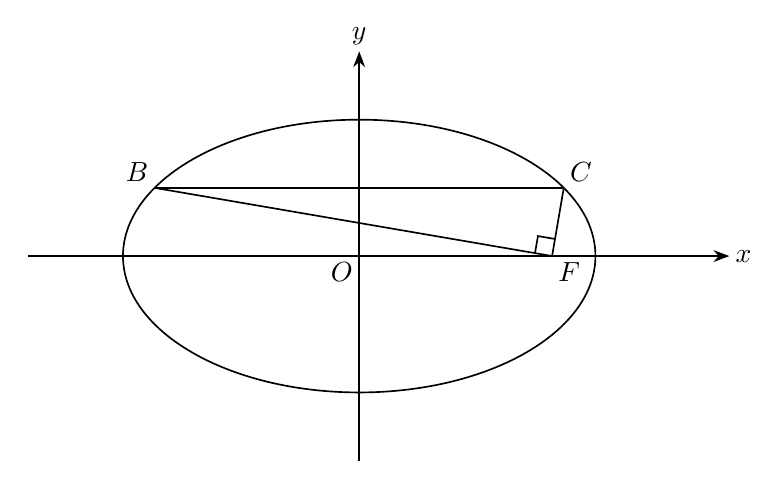
\begin{tikzpicture}[x=1cm,y=1cm,line width=.6pt,font=\normalsize,>=Stealth,
  axis/.style={line width=.6pt},
  curve/.style={line width=.6pt},
  seg/.style={line width=.6pt},
  rightangle/.style={line width=.6pt}]
  \coordinate (O) at (0,0);
  \coordinate (F) at (2.449489743,0);
  \coordinate (B) at (-2.598076211,0.866025404);
  \coordinate (C) at (2.598076211,0.866025404);
  \draw[axis,->] (-4.2,0)--(4.7,0) node[right,inner sep=0pt,xshift=2pt] {$x$};
  \draw[axis,->] (0,-2.6)--(0,2.6) node[above,inner sep=0pt,yshift=2pt] {$y$};
  \draw[curve] (O) ellipse[x radius=3.000000000,y radius=1.732050808];
  \draw[seg] (B)--(C);
  \draw[seg] (F)--(B);
  \draw[seg] (F)--(C);
  \draw[rightangle] (2.232658060,0.037202435)--(2.269860495,0.254034118)--(2.486692178,0.216831683);
  \node[above left,inner sep=2pt] at (B) {$B$};
  \node[above right,inner sep=2pt] at (C) {$C$};
  \node[below right,inner sep=2pt] at (F) {$F$};
  \node[below left,inner sep=2pt] at (O) {$O$};
\end{tikzpicture}
